\documentclass[11pt,compress,t,notes=noshow, xcolor=table]{beamer}
\usepackage[]{graphicx}\usepackage[]{color}
% maxwidth is the original width if it is less than linewidth
% otherwise use linewidth (to make sure the graphics do not exceed the margin)
\makeatletter
\def\maxwidth{ %
  \ifdim\Gin@nat@width>\linewidth
    \linewidth
  \else
    \Gin@nat@width
  \fi
}
\makeatother

\definecolor{fgcolor}{rgb}{0.345, 0.345, 0.345}
\newcommand{\hlnum}[1]{\textcolor[rgb]{0.686,0.059,0.569}{#1}}%
\newcommand{\hlstr}[1]{\textcolor[rgb]{0.192,0.494,0.8}{#1}}%
\newcommand{\hlcom}[1]{\textcolor[rgb]{0.678,0.584,0.686}{\textit{#1}}}%
\newcommand{\hlopt}[1]{\textcolor[rgb]{0,0,0}{#1}}%
\newcommand{\hlstd}[1]{\textcolor[rgb]{0.345,0.345,0.345}{#1}}%
\newcommand{\hlkwa}[1]{\textcolor[rgb]{0.161,0.373,0.58}{\textbf{#1}}}%
\newcommand{\hlkwb}[1]{\textcolor[rgb]{0.69,0.353,0.396}{#1}}%
\newcommand{\hlkwc}[1]{\textcolor[rgb]{0.333,0.667,0.333}{#1}}%
\newcommand{\hlkwd}[1]{\textcolor[rgb]{0.737,0.353,0.396}{\textbf{#1}}}%
\let\hlipl\hlkwb

\usepackage{framed}
\makeatletter
\newenvironment{kframe}{%
 \def\at@end@of@kframe{}%
 \ifinner\ifhmode%
  \def\at@end@of@kframe{\end{minipage}}%
  \begin{minipage}{\columnwidth}%
 \fi\fi%
 \def\FrameCommand##1{\hskip\@totalleftmargin \hskip-\fboxsep
 \colorbox{shadecolor}{##1}\hskip-\fboxsep
     % There is no \\@totalrightmargin, so:
     \hskip-\linewidth \hskip-\@totalleftmargin \hskip\columnwidth}%
 \MakeFramed {\advance\hsize-\width
   \@totalleftmargin\z@ \linewidth\hsize
   \@setminipage}}%
 {\par\unskip\endMakeFramed%
 \at@end@of@kframe}
\makeatother

\definecolor{shadecolor}{rgb}{.97, .97, .97}
\definecolor{messagecolor}{rgb}{0, 0, 0}
\definecolor{warningcolor}{rgb}{1, 0, 1}
\definecolor{errorcolor}{rgb}{1, 0, 0}
\newenvironment{knitrout}{}{} % an empty environment to be redefined in TeX

\usepackage{alltt}
\newcommand{\SweaveOpts}[1]{}  % do not interfere with LaTeX
\newcommand{\SweaveInput}[1]{} % because they are not real TeX commands
\newcommand{\Sexpr}[1]{}       % will only be parsed by R
\newcommand{\xmark}{\ding{55}}%


\usepackage[english]{babel}
\usepackage[utf8]{inputenc}

\usepackage{dsfont}
\usepackage{verbatim}
\usepackage{amsmath}
\usepackage{amsfonts}
\usepackage{amssymb}
\usepackage{bm}
\usepackage{csquotes}
\usepackage{multirow}
\usepackage{longtable}
\usepackage{booktabs}
\usepackage{enumerate}
\usepackage[absolute,overlay]{textpos}
\usepackage{psfrag}
\usepackage{algorithm}
\usepackage{algpseudocode}
\usepackage{eqnarray}
\usepackage{arydshln}
\usepackage{tabularx}
\usepackage{placeins}
\usepackage{tikz}
\usepackage{setspace}
\usepackage{colortbl}
\usepackage{mathtools}
\usepackage{wrapfig}
\usepackage{bm}
\usepackage{amsmath}
\usepackage{pifont}
\usepackage{xcolor} %colored math symbols

\usetikzlibrary{shapes,arrows,automata,positioning,calc,chains,trees, shadows}
\tikzset{
  %Define standard arrow tip
  >=stealth',
  %Define style for boxes
  punkt/.style={
    rectangle,
    rounded corners,
    draw=black, very thick,
    text width=6.5em,
    minimum height=2em,
    text centered},
  % Define arrow style
  pil/.style={
    ->,
    thick,
    shorten <=2pt,
    shorten >=2pt,}
}

\usepackage{subfig}

% Defines macros and environments
\usepackage{../../style/lmu-lecture}


\let\code=\texttt
\let\proglang=\textsf

\setkeys{Gin}{width=0.9\textwidth}

\setbeamertemplate{frametitle}{\expandafter\uppercase\expandafter\insertframetitle}

\usepackage{bbm}
% basic latex stuff
\newcommand{\pkg}[1]{{\fontseries{b}\selectfont #1}} %fontstyle for R packages
\newcommand{\lz}{\vspace{0.5cm}} %vertical space
\newcommand{\dlz}{\vspace{1cm}} %double vertical space
\newcommand{\oneliner}[1] % Oneliner for important statements
{\begin{block}{}\begin{center}\begin{Large}#1\end{Large}\end{center}\end{block}}


%new environments
\newenvironment{vbframe}  %frame with breaks and verbatim
{
 \begin{frame}[containsverbatim,allowframebreaks]
}
{
\end{frame}
}

\newenvironment{vframe}  %frame with verbatim without breaks (to avoid numbering one slided frames)
{
 \begin{frame}[containsverbatim]
}
{
\end{frame}
}

\newenvironment{blocki}[1]   % itemize block
{
 \begin{block}{#1}\begin{itemize}
}
{
\end{itemize}\end{block}
}

\newenvironment{fragileframe}[2]{  %fragile frame with framebreaks
\begin{frame}[allowframebreaks, fragile, environment = fragileframe]
\frametitle{#1}
#2}
{\end{frame}}


\newcommand{\myframe}[2]{  %short for frame with framebreaks
\begin{frame}[allowframebreaks]
\frametitle{#1}
#2
\end{frame}}

\newcommand{\remark}[1]{
  \textbf{Remark:} #1
}


\newenvironment{deleteframe}
{
\begingroup
\usebackgroundtemplate{
\includegraphics[width=\paperwidth,height=\paperheight]{../style/color/red.png}}
 \begin{frame}
}
{
\end{frame}
\endgroup
}
\newenvironment{simplifyframe}
{
\begingroup
\usebackgroundtemplate{
\includegraphics[width=\paperwidth,height=\paperheight]{../style/color/yellow.png}}
 \begin{frame}
}
{
\end{frame}
\endgroup
}\newenvironment{draftframe}
{
\begingroup
\usebackgroundtemplate{
\includegraphics[width=\paperwidth,height=\paperheight]{../style/color/green.jpg}}
 \begin{frame}
}
{
\end{frame}
\endgroup
}
% https://tex.stackexchange.com/a/261480: textcolor that works in mathmode
\makeatletter
\renewcommand*{\@textcolor}[3]{%
  \protect\leavevmode
  \begingroup
    \color#1{#2}#3%
  \endgroup
}
\makeatother


\input{../../latex-math/basic-math}
\input{../../latex-math/basic-ml}
\input{../../latex-math/ml-nn}

\newcommand{\titlefigure}{figure/momentum.png}
\newcommand{\learninggoals}{
  \item 
  \item 
  \item 
}

\title{Deep Learning}
\date{}

\begin{document}

\lecturechapter{Advanced Optimization}
\lecture{I2DL}

%%%%%%%%%%%%%%%%%%%%%%%%%%%%%%%%%%%%%%%%%%%%%%%%%%%%%%%%%%%%%%%%%%
\section{Momentum}
%%%%%%%%%%%%%%%%%%%%%%%%%%%%%%%%%%%%%%%%%%%%%%%%%%%%%%%%%%%%%%%%%%
\begin{vbframe}{Momentum}
  \begin{itemize}
    \item While SGD remains a popular optimization strategy, learning with it can sometimes be slow. 
    \item Momentum is designed to accelerate learning, especially when facing high curvature, small but consistent or noisy gradients.
    \item Momentum accumulates an exponentially decaying moving average of past gradients:
      \begin{eqnarray*} 
        \nub &\leftarrow& \varphi \nub - \alpha \underbrace{\nabla_{\thetab} \Big[\frac{1}{m} \sum_{i} \Lmomentum \Big]}_{\mathbf{g}_{\thetab}}\\[-0.3cm]
        \thetab &\leftarrow& \thetab + \nub
      \end{eqnarray*}
    \item We introduce a new hyperparameter $\varphi \in [0, 1)$, determining how quickly the contribution of previous gradients decay.
    \item $\nub$ is called \enquote{velocity} and derives from a physical analogy describing how particles move through a parameter space (Newton's law of motion).
  \end{itemize}
\end{vbframe}

%%%%%%%%%%%%%%%%%%%%%%%%%%%%%%%%%%%%%%%%%%%%%%%%%%%%%%%%%%%%%%%%%%
%%%%%%%%%%%%%%%%%%%%%%%%%%%%%%%%%%%%%%%%%%%%%%%%%%%%%%%%%%%%%%%%%%
\begin{vbframe}{Momentum}
  \begin{itemize}
    \item So far the step size was simply the gradient $\mathbf{g}$ multiplied by the learning rate $\alpha$.
    \item Now, the step size depends on how \textbf{large} and how \textbf{aligned} a sequence of gradients is. The step size grows when many successive gradients point in the same direction.
    \item Common values for $\varphi$ are $0.5, 0.9$ and even $0.99$.
    \item Generally, the larger $\varphi$ is relative to the learning rate $\alpha$, the more previous gradients affect the current direction.
    \item A very good website with an in-depth analysis of momentum: \url{https://distill.pub/2017/momentum/}

\end{itemize}
\end{vbframe}

%%%%%%%%%%%%%%%%%%%%%%%%%%%%%%%%%%%%%%%%%%%%%%%%%%%%%%%%%%%%%%%%%%
%%%%%%%%%%%%%%%%%%%%%%%%%%%%%%%%%%%%%%%%%%%%%%%%%%%%%%%%%%%%%%%%%%
\begin{vbframe}{Momentum: Example}
  \footnotesize 
  \begin{eqnarray*}
    \nu_{1} &\leftarrow& \varphi \nu_0 - \alpha g(\theta^{[0]}) \\[0.1cm]
    \theta^{[1]} &\leftarrow& \theta^{[0]} + \varphi \nu_0 - \alpha g(\theta^{[0]}) \\[0.1cm]
    \nu_{2} &\leftarrow& \varphi \nu_1 - \alpha g(\theta^{[1]}) \\
            &=& \varphi (\varphi \nu_0 - \alpha g(\theta^{[0]})) - \alpha g(\theta^{[1]}) \\[0.1cm]
    \theta^{[2]} &\leftarrow& \theta^{[1]} + \varphi (\varphi \nu_0 - \alpha g(\theta^{[0]})) - \alpha g(\theta^{[1]}) \\[0.1cm]
    \nu_{3} &\leftarrow& \varphi \nu_2 - \alpha g(\theta^{[2]}) \\
            &=& \varphi (\varphi (\varphi \nu_0 - \alpha g(\theta^{[0]})) - \alpha g(\theta^{[1]})) - \alpha g(\theta^{[2]}) \\[0.1cm]
    \theta^{[3]} &\leftarrow& \theta^{[2]} + \varphi (\varphi (\varphi \nu_0 - \alpha g(\theta^{[0]})) - \alpha g(\theta^{[1]})) - \alpha g(\theta^{[2]}) \\
            &=& \theta^{[2]} + \varphi^3\nu_0 - \varphi^2\alpha g(\theta^{[0]}) - \varphi \alpha g(\theta^{[1]}) - \alpha g(\theta^{[2]}) \\
            &=& \theta^{[2]} - \alpha(\varphi^2g(\theta^{[0]}) + \varphi^1g(\theta^{[1]}) + \varphi^0g(\theta^{[2]})) + \varphi^3 \nu_0 \\
\theta^{[t+1]} &=& \theta^{[t]} - \alpha \displaystyle\sum_{j = 0}^{t} \varphi^j g(\theta^{[t - j]}) + \varphi^{t+1}\nu_0
  \end{eqnarray*}
%\framebreak
Suppose momentum always observes the same gradient $g(\theta)$:
  \footnotesize 
  \begin{eqnarray*}
    \theta^{[t+1]} &=& \theta^{[t]} - \alpha \displaystyle\sum_{j = 0}^{t} \varphi^j g(\theta^{[j]}) + \varphi^{t+1}\nu_0 \\
                 &=& \theta^{[t]} - \alpha g(\theta) \displaystyle\sum_{j = 0}^{t} \varphi^j + \varphi^{t+1}\nu_0 \\
                 &=& \theta^{[t]} - \alpha g(\theta) \frac{1 - \varphi^{t+1}}{1 - \varphi} + \varphi^{t+1} \nu_0 \\
                 &\to& \theta^{[t]} - \alpha g(\theta) \frac{1}{1 - \varphi} \qquad \text{ for } t \to \infty. 
  \end{eqnarray*}

Thus, momentum will accelerate in the direction of $-g(\theta)$ until reaching terminal velocity with step size: 
    $$-\alpha g(\theta)(1 + \varphi + \varphi^2 + \varphi^3 + ...) = -\alpha g(\theta) \frac{1}{1 - \varphi}$$
E.g. a momentum with $\varphi = 0.9$ corresponds to multiplying the maximum speed by 10 relative to the gradient descent algorithm. 
\end{vbframe}


%%%%%%%%%%%%%%%%%%%%%%%%%%%%%%%%%%%%%%%%%%%%%%%%%%%%%%%%%%%%%%%%%%
\begin{frame} {Momentum: Illustration}
     The vector $\nu_{3}$ (for $ \nu_0 = 0$):  \begin{eqnarray*} \nu_{3} &=& \varphi (\varphi (\varphi \nu_0 - \alpha g(\theta^{[0]})) - \alpha g(\theta^{[1]})) - \alpha g(\theta^{[2]}) \\ &=& - \varphi^2 (\alpha g(\theta^{[0]})) - \varphi (\alpha g(\theta^{[1]})) - \alpha g(\theta^{[2]}) \end{eqnarray*}
  \begin{figure}
    \centering
      \scalebox{0.90}{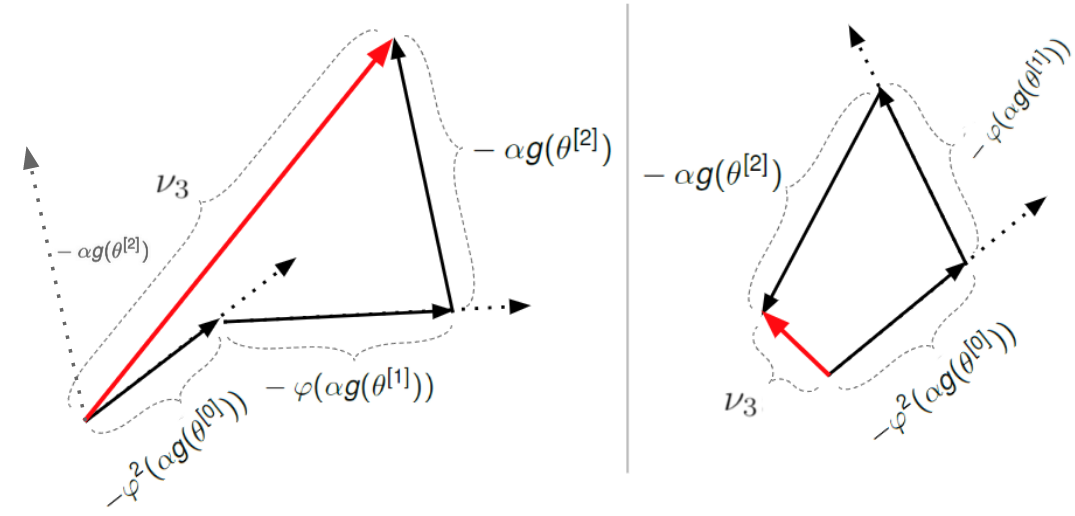
\includegraphics{figure/moment_vis2.png}}
      \caption{\footnotesize{If consecutive (negative) gradients point mostly in the same direction, the velocity "builds up". On the other hand, if consecutive (negative) gradients point in very different directions, the velocity "dies down".}}
    \end{figure}
\end{frame}

%%%%%%%%%%%%%%%%%%%%%%%%%%%%%%%%%%%%%%%%%%%%%%%%%%%%%%%%%%%%%%%%%%

\begin{vbframe}{SGD with momentum}
  \begin{algorithm}[H]
  \small
    \caption{Stochastic gradient descent with momentum}
    \begin{algorithmic}[1]
    \State \textbf{require} learning rate $\alpha$ and momentum $\varphi$ \strut
    \State \textbf{require} initial parameter $\thetab$ and initial velocity $\nub$ \strut
      \While{stopping criterion not met}
        \State \parbox[t]{\dimexpr\linewidth-\algorithmicindent}{Sample a minibatch of $m$ examples from the training set $\{\tilde{x}^{(1)},\dots,\tilde{x}^{(m)}\}$}
        \State Compute gradient estimate: $\hat{\mathbf{g}} \leftarrow  \frac{1}{m} \nabla_{\thetab} \sum_{i} \Lxym$
        \State Compute velocity update: $\nub \leftarrow \varphi \nub - \alpha \hat{\mathbf{g}}$
        \State Apply update: $\thetab \leftarrow \thetab + \nub$
      \EndWhile
    \end{algorithmic}
  \end{algorithm}
  
\framebreak
  
  \begin{figure}
  \captionsetup{font=footnotesize,labelfont=footnotesize, labelfont = bf}
  \centering
    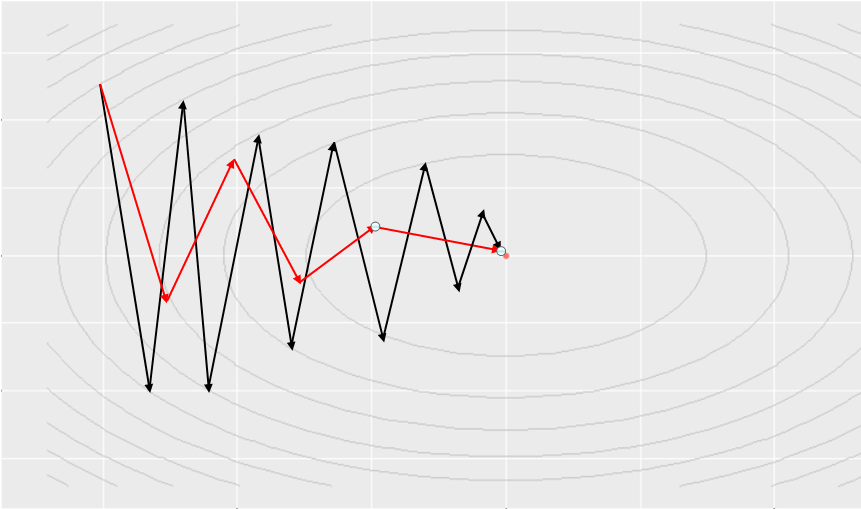
\includegraphics[height = 6 cm, width = 10 cm]{figure/momentum.png}
    \caption{The contour lines show a quadratic loss function with a poorly conditioned Hessian matrix. The two curves show how standard gradient descent (black) and momentum (red) learn when dealing with ravines. Momentum reduces the oscillation and accelerates the convergence.}
  \end{figure}
\end{vbframe}

%%%%%%%%%%%%%%%%%%%%%%%%%%%%%%%%%%%%%%%%%%%%%%%%%%%%%%%%%%%%%%%%%%
%%%%%%%%%%%%%%%%%%%%%%%%%%%%%%%%%%%%%%%%%%%%%%%%%%%%%%%%%%%%%%%%%%
\begin{vbframe}{SGD with and without momentum}
\footnotesize The following plot was created by our Shiny App. On the upper left you can explore different predefined examples. \href{https://juliambr.shinyapps.io/shinyapp/}{\beamergotobutton{Click here}}
\begin{figure}
\vspace{-0.3cm}
  \captionsetup{font=footnotesize,labelfont=footnotesize, labelfont = bf}
  \centering
    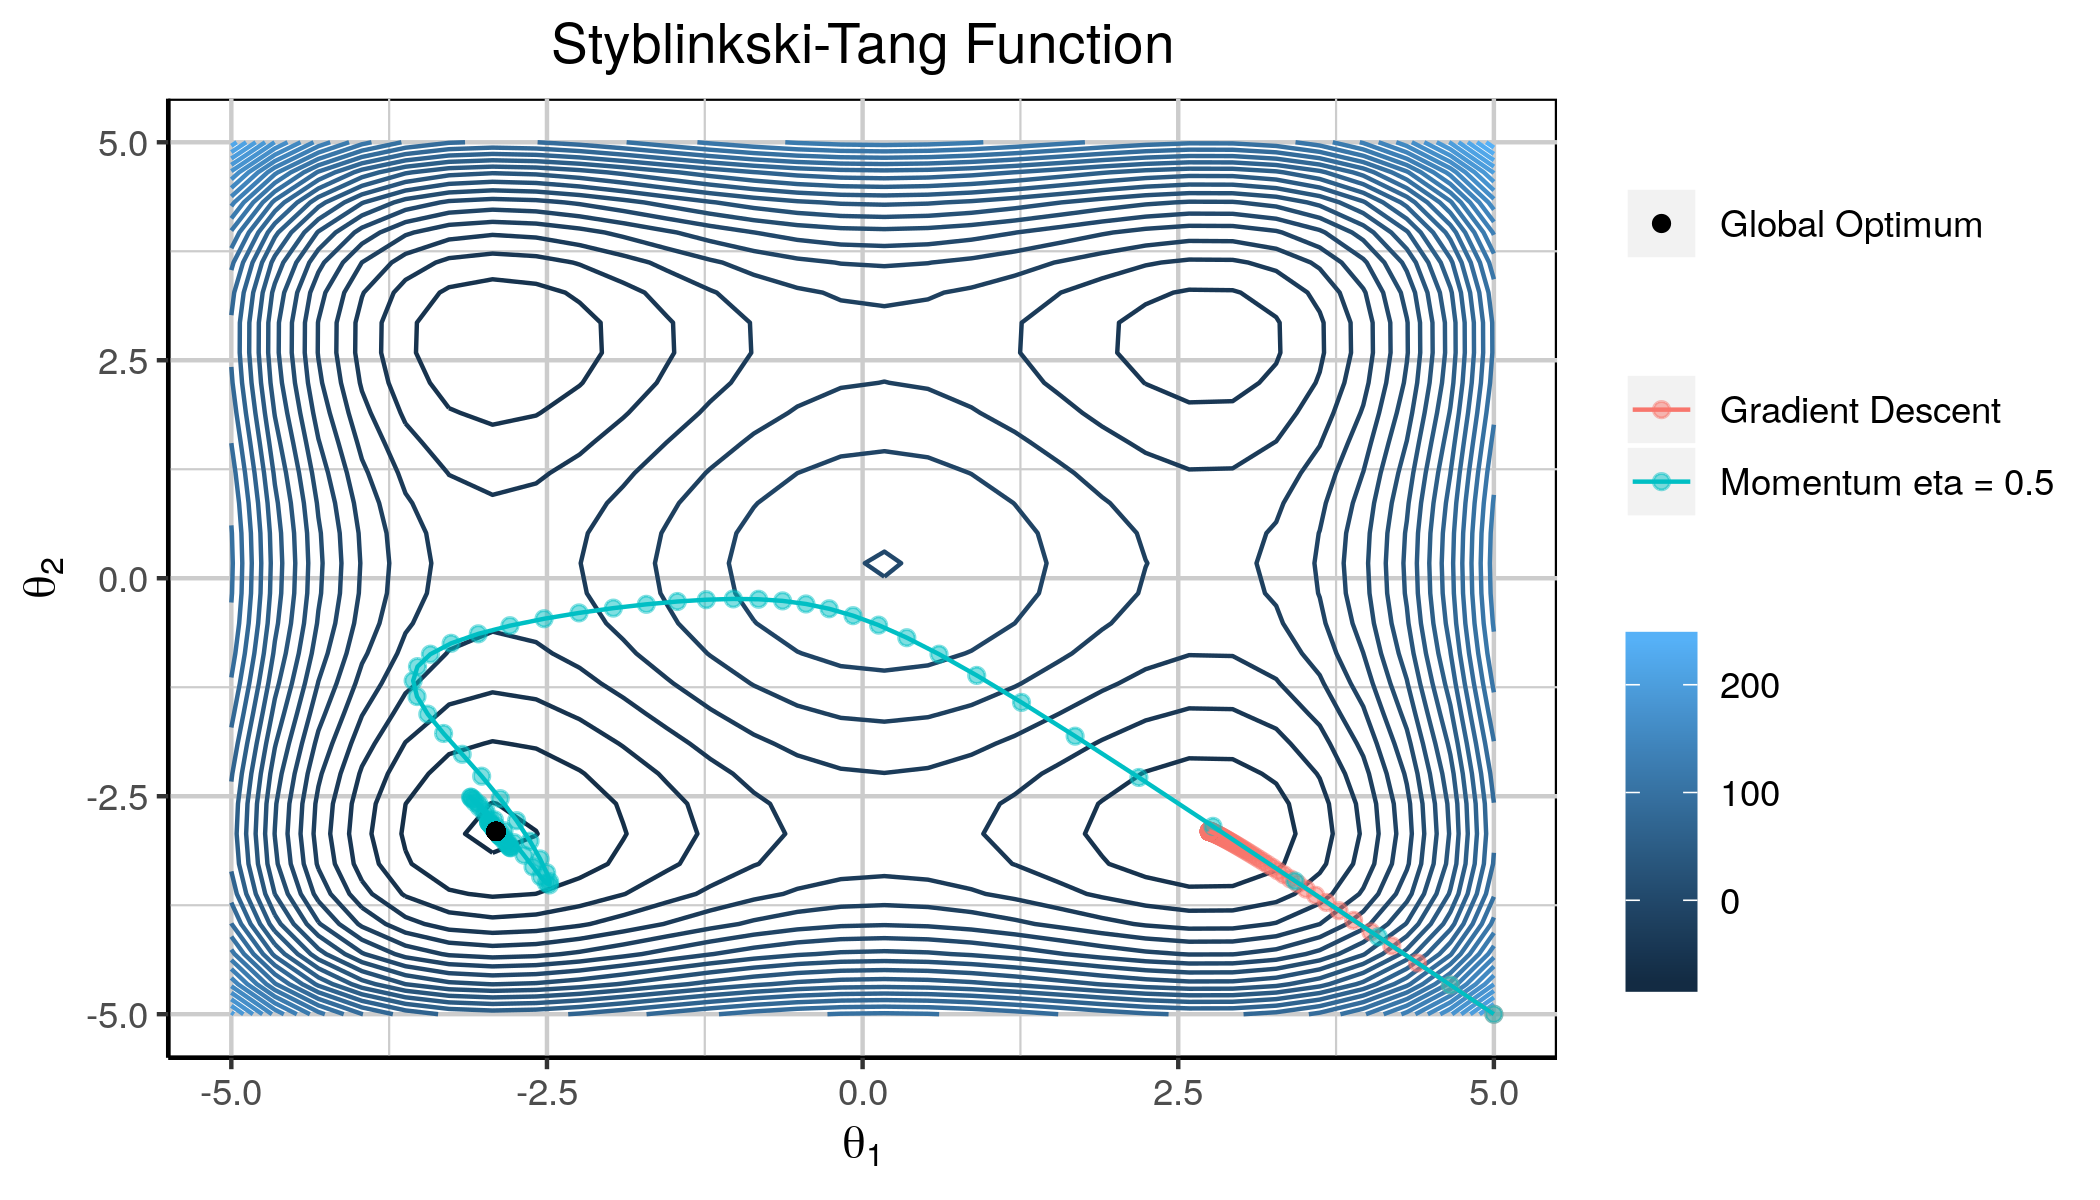
\includegraphics[width = 8cm]{figure/momentum2.png}
    \caption{Comparison of SGD with and without momentum on the Styblinkski-Tang function.
    The black dot on the bottom left is the global optimum. We can see that 
    SGD without momentum (red line/points) cannot escape the local minimum, while SGD with momentum (blue line/dots) is able to escape the local minimum and finds the global minimum.}
  \end{figure}
\end{vbframe}

%%%%%%%%%%%%%%%%%%%%%%%%%%%%%%%%%%%%%%%%%%%%%%%%%%%%%%%%%%%%%%%%%%
%%%%%%%%%%%%%%%%%%%%%%%%%%%%%%%%%%%%%%%%%%%%%%%%%%%%%%%%%%%%%%%%%%
\begin{vbframe}{Momentum in practice}
  \begin{minipage}{0.5\textwidth}
  \begin{itemize}
    \item Lets try out different values of momentum (with SGD) on the MNIST data.
    \item We apply the same architecture we have used a dozen of times already (note that we used $\varphi = 0.9$ in all computations so far, i.e. in chapter 1 and 2)!
  \end{itemize}
  \end{minipage}
  \begin{minipage}{0.3\textwidth}


  \begin{figure}
  \begin{flushleft}
      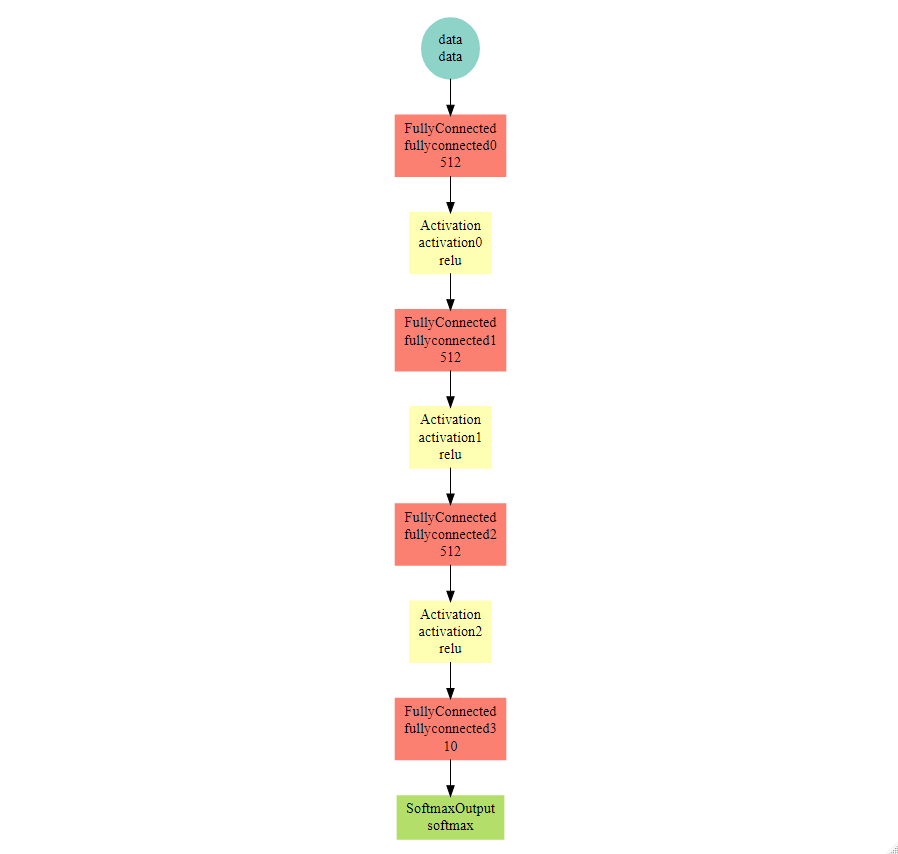
\includegraphics[width=8.6cm]{figure/mxnet_graph.png}
    \end{flushleft}
  \end{figure}
\end{minipage}
\end{vbframe}
\begin{vbframe}{Momentum in practice}
  \begin{figure}
  \begin{center}
    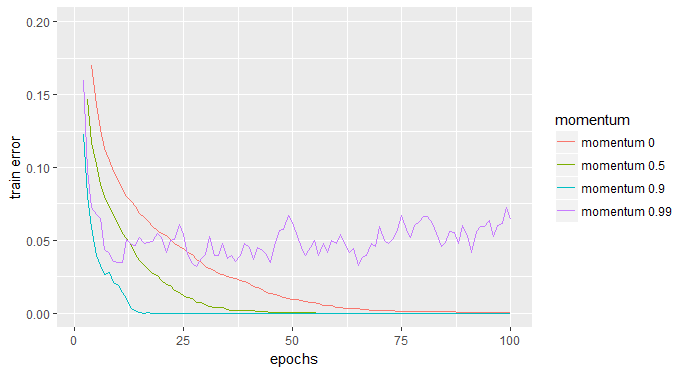
\includegraphics[width=10.5cm]{figure/momentum_train.png}
    \end{center}
  \end{figure}
    \small{The higher momentum, the faster SGD learns the weights on the training data, but if momentum is too large, the training and test error fluctuates.}

\framebreak

  \begin{figure}
  \centering
    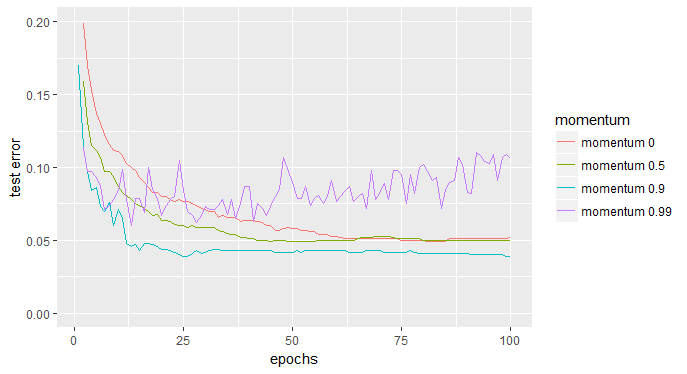
\includegraphics[width=10.5cm]{figure/momentum_test.png}
  \end{figure}
      \small{The higher momentum, the faster SGD learns the weights on the training data, but if momentum is too large, the training and test error fluctuates.}
\end{vbframe}


\begin{vbframe}{Nesterov momentum}
  \begin{itemize}
    \item Momentum aims to solve poor conditioning of the Hessian but also variance in the stochastic gradient.
    \item Nesterov momentum modifies the algorithm such that the gradient is evaluated after the current velocity is applied:
      \begin{eqnarray*} 
        \nub &\leftarrow& \varphi \nub - \alpha \nabla_{\thetab} \Big[\frac{1}{m} \sum_{i} \Lmomentumnest \Big] \\
        \thetab &\leftarrow& \thetab + \nub
      \end{eqnarray*}
    \item We can interpret Nesterov momentum as an attempt to add a correction factor to the basic method.
    \item The method is also called Nesterov accelerated gradient (NAG).
  \end{itemize}
\end{vbframe}

\begin{vbframe}{SGD with Nesterov Momentum}
  \begin{algorithm}[H]
  \small
    \caption{Stochastic gradient descent with Nesterov momentum}
    \begin{algorithmic}[1]
    \State \textbf{require} learning rate $\alpha$ and momentum $\varphi$ \strut
    \State \textbf{require} initial parameter $\thetab$ and initial velocity $\nub$ \strut
      \While{stopping criterion not met}
        \State \parbox[t]{\dimexpr\linewidth-\algorithmicindent}{Sample a minibatch of $m$ examples from the training set $\{\tilde{x}^{(1)},\dots,\tilde{x}^{(m)}\}$}
        \State Apply interim update: $\tilde{\thetab} \leftarrow \thetab + \varphi \nub$
        \State Compute gradient estimate: $\hat{\mathbf{g}} \leftarrow  \frac{1}{m} \nabla_{\tilde{\thetab}} \sum_{i} \Lmomentumtilde$
        \State Compute velocity update: $\nub \leftarrow \varphi \nub - \alpha \hat{\mathbf{g}}$
        \State Apply update: $\thetab \leftarrow \thetab + \nub$
      \EndWhile
    \end{algorithmic}
  \end{algorithm}
\end{vbframe}


\begin{vbframe}{Momentum vs. Nesterov Momentum}
  \begin{figure}
   \vspace{-0.3cm}
  \captionsetup{font=footnotesize,labelfont=footnotesize, labelfont = bf}
    \centering
      \scalebox{0.90}{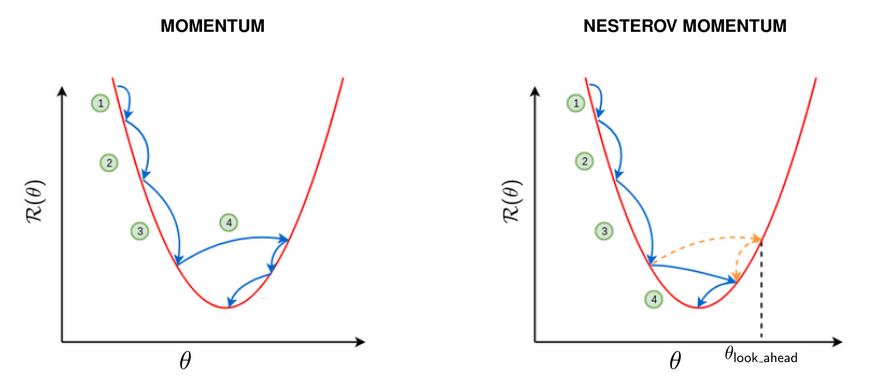
\includegraphics{figure/nesterov_momentum.png}}
      \tiny{\\Credits: Chandra (2015)}
      \caption{\footnotesize{Comparison GD with momentum (left) and GD with Nesterov momentum (right) for one parameter $\theta$. The first three updates of $\theta$ are very similar in both cases and the updates become larger due to momentum (accumulation of previous negative gradients). Update 4 is different. In case of momentum, the update overshoots as it makes an even bigger step due to the gradient history. In contrast, Nesterov momentum first evaluates a "look-ahead" point $\theta_{\text{look\_ahead}}$, detects that it overshoots, and slightly reduces the overall magnitude of the fourth update. Thus, Nesterov momentum reduces overshooting and leads to smaller oscillations than momentum. }}
    \end{figure}
\end{vbframe}

%%%%%%%%%%%%%%%%%%%%%%%%%%%%%%%%%%%%%%%%%%%%%%%%%%%%%%%%%%%%%%%%%%

\section{Learning Rates}

\begin{frame} {Learning Rate}
  \begin{itemize}
    \item The learning rate is a very important hyperparameter.
    \item To systematically find a good learning rate, we can start at a very low learning rate and gradually increase it (linearly or exponentially) after each mini-batch.
    \item We can then plot the learning rate and the training loss for each batch.
    \item A good learning rate is one that results in a steep decline in the loss.
    \begin{figure}
    \centering
      \scalebox{0.7}{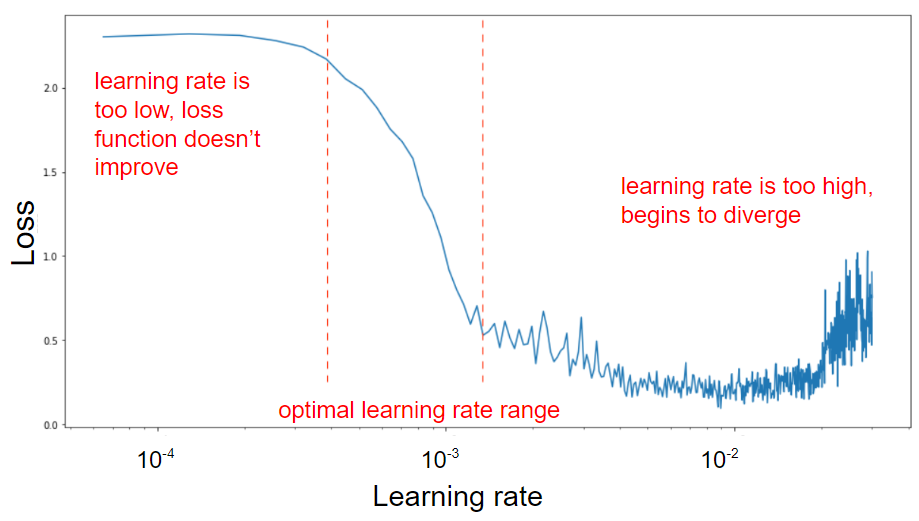
\includegraphics{figure/lr_jh.png}}
      \tiny{\\Credit: jeremyjordan}
    \end{figure}
  \end{itemize}
\end{frame}

%%%%%%%%%%%%%%%%%%%%%%%%%%%%%%%%%%%%%%%%%%%%%%%%%%%%%%%%%%%%%%%%%%

% the code below produces the same results but looks alot worse since 
% knitr is very stupid and makes figure jumping around

%\begin{vbframe}{Example: saddle point}
%   \begin{center}
%     $f(x_1, x_2) = x_1^2 - x_2^2$
% <<opt1, size = "small", echo=FALSE, fig.width=6, fig.height=3.5, eval = TRUE>>=
% foo = function(x, y){
%   x^2 - y^2
% }
% x = y = seq(-1.6, 1.6, length = 30)
% z = outer(x, y, foo)
% p = c(list(list(1, 0)), optim0(.2, 0, FUN = foo, maximum = FALSE, maxit = 1))
% #p = c(list(list(-100, 100)))
% sd_plot(phi = 40, theta = 320, xlab = "x1", ylab = "x2")
% @
%     Starting point
%   \end{center}
% \framebreak
%   \begin{center}
%     $f(x_1, x_2) = x_1^2 - x_2^2$
% <<opt2, size = "small", echo=FALSE, fig.width=6, fig.height=3.5, eval = TRUE>>=
% foo = function(x, y){
%   x^2 - y^2
% }
% x = y = seq(-1.6, 1.6, length = 30)
% z = outer(x, y, foo)
% p = c(list(list(1, 0)), optim0(.2, 0, FUN = foo, maximum = FALSE, maxit = 2))
% #p = c(list(list(-100, 100)))
% sd_plot(phi = 40, theta = 320, xlab = "x1", ylab = "x2")
% @
%     First step
%   \end{center}
% \framebreak
%   \begin{center}
%     $f(x_1, x_2) = x_1^2 - x_2^2$  
% <<opt3, echo=FALSE, fig.width=8, fig.height=4>>=
% foo = function(x, y){
%   x^2 - y^2
% }
% x = y = seq(-1.6, 1.6, length = 30)
% z = outer(x, y, foo)
% p = c(list(list(1, 0)), optim0(.2, 0, FUN = foo, maximum = FALSE, maxit = 3))
% #p = c(list(list(-100, 100)))
% sd_plot(phi = 40, theta = 320, xlab = "x1", ylab = "x2")
% @
%     Second step
%   \end{center}
% \framebreak
%   \begin{center}
%     $f(x_1, x_2) = x_1^2 - x_2^2$
% <<opt4, echo=FALSE, fig.width=8, fig.height=4>>=
% foo = function(x, y){
%   x^2 - y^2
% }
% x = y = seq(-1.6, 1.6, length = 30)
% z = outer(x, y, foo)
% p = c(list(list(1, 0)), optim0(.2, 0, FUN = foo, maximum = FALSE, maxit = 10))
% #p = c(list(list(-100, 100)))
% sd_plot(phi = 40, theta = 320, xlab = "x1", ylab = "x2")
% @
%     Tenth step
%   \end{center}
%\end{vbframe}
%%%%%%%%%%%%%%%%%%%%%%%%%%%%%%%%%%%%%%%%%%%%%%%%%%%%%%%%%%%%%%%%%%
%%%%%%%%%%%%%%%%%%%%%%%%%%%%%%%%%%%%%%%%%%%%%%%%%%%%%%%%%%%%%%%%%%
%%%%%%%%%%%%%%%%%%%%%%%%%%%%%%%%%%%%%%%%%%%%%%%%%%%%%%%%%%%%%%%%%%
%%%%%%%%%%%%%%%%%%%%%%%%%%%%%%%%%%%%%%%%%%%%%%%%%%%%%%%%%%%%%%%%%%
% \begin{vbframe}{Local minima}
%   \begin{itemize}
%     \item Convex optimization problems can be reduced to \enquote{finding a local minimum}.
%       \begin{itemize}
%         \item Any local minimum is a global minimum!
%       \end{itemize}
%     \item In neural networks we have to deal with non-convex problems.
%       \begin{itemize}
%         \item Generally, we have many saddle points!
%         \item Nearly any deep network is guaranteed to have an extremely large amount of saddle points.
%       \end{itemize}
%     \item In practice, nearly all difficulty with neural network optimization arises from local minima.
%       \begin{itemize}
%         \item To test if stuck in a local minina one could plot the norm of the gradient over time.
%         \item If it does not shrink to insignificant size, the problem is neither local minima nor any other kind of critical point.
%       \end{itemize}
%   \end{itemize}
% \end{vbframe}
%%%%%%%%%%%%%%%%%%%%%%%%%%%%%%%%%%%%%%%%%%%%%%%%%%%%%%%%%%%%%%%%%%

\begin{vbframe}{Learning Rate Schedule}
  \begin{itemize}
    \item We would like to force convergence until reaching a local minimum.
    \item Applying SGD, we have to decrease the learning rate over time, thus $\alpha^{[t]}$ (learning rate at training iteration $t$).
      \begin{itemize}
        \item The estimator $\hat{\mathbf{g}}$ is computed based on small batches.
        \item Random sampling $m$ training samples introduces noise, that does not vanish even if we find a minimum.
      \end{itemize}
    \item In practice, a common strategy is to decay the learning rate linearly over time until iteration $\tau$:
         \begin{equation*}
         \alpha^{[t]} = \begin{cases}
         \left( 1 - \frac{t}{\tau} \right)\alpha^{[0]} + \frac{t}{\tau}\alpha^{[\tau]}
                    = t\left(-\frac{\alpha^{[0]} +  \alpha^{[\tau]}}{\tau}\right) + \alpha^{[0]} & 
                    \text{for $t\le\tau$} \\
                    \alpha^{[\tau]} & \text{for $t>\tau$} \end{cases}
         \end{equation*}
  \end{itemize}
  
\framebreak


\scriptsize Example for $\tau = 4$:
\begin{minipage}{\linewidth}
\centering
  \begin{center}
        {\footnotesize
        \begin{tabular}{l | c | c}
        iteration t &  $t/\tau$ & $\alpha^{[t]}$ \\ \hline
        \multicolumn{1}{c|}{$1$}       
        & $0.25$  
        & $\left(1-\frac{1}{4}\right)\alpha^{[0]} + \frac{1}{4}\alpha^{[\tau]} = \frac{3}{4}\alpha^{[0]} + \frac{1}{4}\alpha^{[\tau]}$\\
        
        \multicolumn{1}{c|}{$2$}       
        & $0.5$   
        & $\frac{2}{4}\alpha^{[0]} + \frac{2}{4}\alpha^{[\tau]}$ \\
        
        \multicolumn{1}{c|}{$3$}       
        & $0.75$  
        & $\frac{1}{4}\alpha^{[0]} + \frac{3}{4}\alpha^{[\tau]}$ \\
        
        \multicolumn{1}{c|}{$4$}       
        & $1$     
        & 0 + $\alpha^{[\tau]}$ \\
        
        \multicolumn{1}{c|}{$...$}       
        &      
        & $\alpha^{[\tau]}$ \\
        
        \multicolumn{1}{c|}{$t+1$}     
        & 
        & $\alpha^{[\tau]} $
        \end{tabular}
        }
  \end{center}
\end{minipage}
  \begin{figure}
  \centering
    \scalebox{0.95}{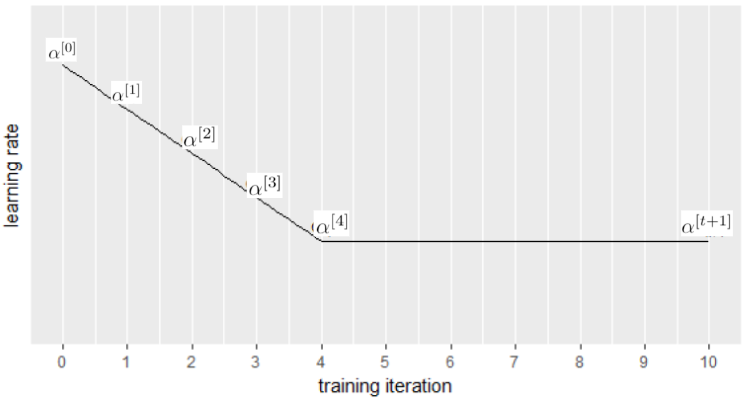
\includegraphics[width=8cm]{figure/weight_decayy.png}}
  \end{figure}
\end{vbframe}

%%%%%%%%%%%%%%%%%%%%%%%%%%%%%%%%%%%%%%%%%%%%%%%%%%%%

\begin{frame} {Cyclical Learning Rates}
  \begin{itemize}
    \item Another option is to have a learning rate that periodically varies according to some cyclic function.
    \item Therefore, if training does not improve the loss anymore (possibly due to saddle points), increasing the learning rate makes it possible to rapidly traverse such regions.
    \item Recall, saddle points are far more likely than local minima in deep nets.
    \item Each cycle has a fixed length in terms of the number of iterations. 
  \end{itemize}
\end{frame}


\begin{frame} {Cyclical Learning Rates}
  \begin{itemize}
    \item One such cyclical function is the "triangular" function.
    \begin{figure}
      \centering
        \scalebox{1}{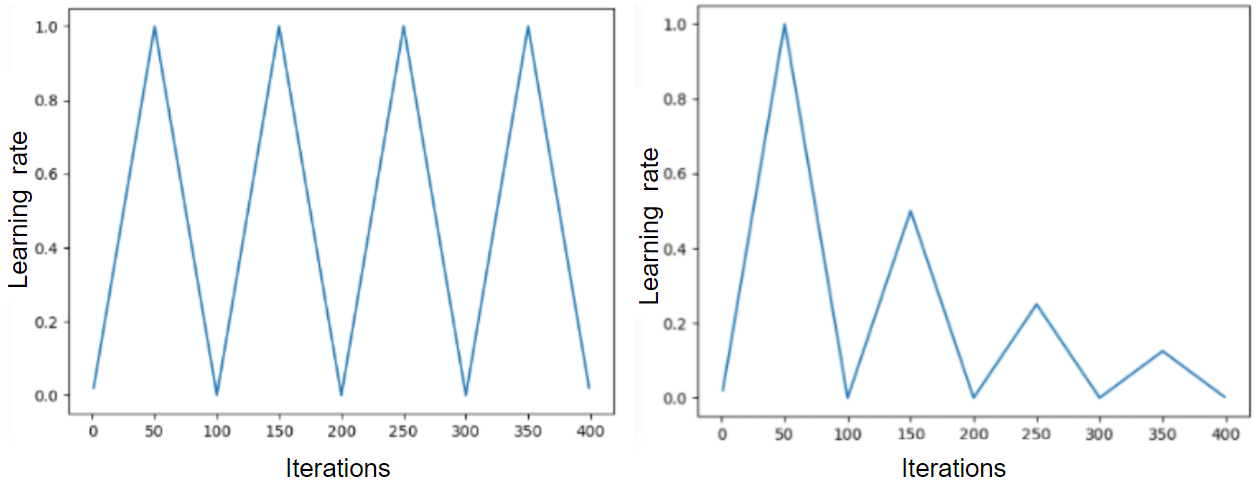
\includegraphics{figure/cyc_triangular.png}}
        \tiny{\\Credit: Hafidz Zulkifli}
    \end{figure}
    \item In the right image, the range is cut in half after each cycle.
  \end{itemize}
\end{frame}


\begin{frame} {Cyclical Learning Rates}
  \begin{itemize}
    \item Yet another option is to abruptly "restart" the learning rate after a fixed number of iterations. 
    \item Loshchilov et al. (2016) proposed  "cosine annealing" (between restarts).
    \begin{figure}
      \centering
        \scalebox{0.6}{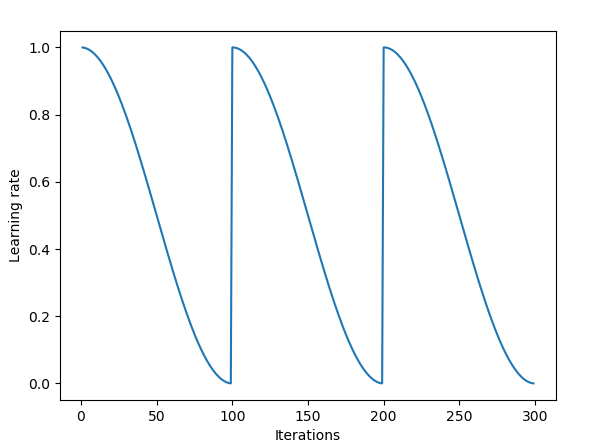
\includegraphics{figure/cyc_cosine.png}}
        \tiny{\\Credit: Hafidz Zulkifli}
    \end{figure}
  \end{itemize}
\end{frame}


%%%%%%%%%%%%%%%%%%%%%%%%%%%%%%%%%%%%%%%%%%%%%%%%%%%%%%%%%%%%%%%%%%
\section{Algorithms with Adaptive Learning Rates}

\begin{vbframe}{Adaptive learning rates}
  \begin{itemize}
    \item The learning rate is reliably one of the hyperparameters that is the most difficult to set because it has a significant impact on the models performance.
    \item Naturally, it might make sense to use a different learning rate for each parameter, and automatically adapt them throughout the training process.
  \end{itemize}
\end{vbframe}
%%%%%%%%%%%%%%%%%%%%%%%%%%%%%%%%%%%%%%%%%%%%%%%%%%%%%%%%%%%%%%%%%%

\begin{vbframe}{Adagrad}
  \begin{itemize}
    \item Adagrad adapts the learning rate to the parameters.
    \item In fact, Adagrad scales learning rates inversely proportional to the square root of the sum of the past squared derivatives.
      \begin{itemize}
        \item Parameters with large partial derivatives of the loss obtain a rapid decrease in their learning rate.
        \item Parameters with small partial derivatives on the other hand obtain a relatively small decrease in their learning rate.
      \end{itemize}
    \item For that reason, Adagrad might be well suited when dealing with sparse data. 
    \item Goodfellow et al. (2016) say that the accumulation of squared gradients can result in a premature and overly decrease in the learning rate.
  \end{itemize}
  
\framebreak
  
  
  \begin{algorithm}[H]
    \small
    \caption{Adagrad}
    \begin{algorithmic}[1]
    \scriptsize 
    \State \textbf{require} Global learning rate $\alpha$ \strut
    \State \textbf{require} Initial parameter $\thetab$ \strut
    \State \textbf{require} Small constant $\beta$, perhaps $10^{-7}$, for numerical stability \strut
    \State \textbf{Initialize} gradient accumulation variable $r = 0$
       \While{stopping criterion not met}
         \State \parbox[t]{\dimexpr\linewidth-\algorithmicindent}{Sample a minibatch of $m$ examples from the training set $\{\tilde{x}^{(1)},\dots,\tilde{x}^{(m)}\}$ \strut}
         \State Compute gradient estimate: $\hat{\mathbf{g}} \leftarrow \frac{1}{m} \nabla_{\thetab} \sum_{i} \Lxym$
         \State Accumulate squared gradient $\mathbf{r} \leftarrow \mathbf{r} + \hat{\mathbf{g}} \odot  \hat{\mathbf{g}}$
         \State \parbox[t]{\dimexpr\linewidth-\algorithmicindent}{Compute update: $\nabla \thetab = - \frac{\alpha}{\beta + \sqrt\mathbf{r}} \odot \hat{\mathbf{g}}$ (division and square root applied element-wise) \strut}
         \State Apply update: $\thetab \leftarrow \thetab + \nabla\thetab$
       \EndWhile
    \end{algorithmic}
  \end{algorithm}
  \begin{itemize}
  \small
    \item \enquote{$\odot$} is called Hadamard or element-wise product.
    \item Example:
    \vspace{0.2cm}
    \item[] $A =
            \begin{bmatrix}
              1 & 2 \\
              3 & 4
            \end{bmatrix}, \ 
            B =
            \begin{bmatrix}
              5 & 6 \\
              7 & 8
            \end{bmatrix}, \ \text{ then } A \odot B =
            \begin{bmatrix}
              1 \cdot 5 & 2 \cdot 6 \\
              3 \cdot 7 & 4 \cdot 8
            \end{bmatrix}$
  \end{itemize}
\end{vbframe}

%%%%%%%%%%%%%%%%%%%%%%%%%%%%%%%%%%%%%%%%%%%%%%%%%%%%%%%%%%%%%%%%%%

\begin{vbframe}{RMSProp}
  \begin{itemize}
    \item RMSprop is a modification of Adagrad.
    \item It's intention is to resolve Adagrad's radically diminishing learning rates.
    \item The gradient accumulation is replaced by an exponentially weighted moving average.
    \item Theoretically, that leads to performance gains in non-convex scenarios.
    \item Empirically, RMSProp is a very effective optimization algorithm. Particularly, it is employed routinely by deep learning practitioners.
  \end{itemize}
  
\framebreak
  
  
  \begin{algorithm}[H]
    \small
    \caption{RMSProp}
    \begin{algorithmic}[1]
    \State \textbf{require} Global learning rate $\alpha$ and decay rate $\rho$ \strut
    \State \textbf{require} Initial parameter $\mathbf{\thetab}$ \strut
    \State \parbox[t]{\dimexpr\linewidth-\algorithmicindent}{\textbf{require} Small constant $\beta$, perhaps $10^{-6}$, to stabilize division by small numbers \strut}
    \State Initialize gradient accumulation variable $r = 0$
      \While{stopping criterion not met}
        \State \parbox[t]{\dimexpr\linewidth-\algorithmicindent}{Sample a minibatch of $m$ examples from the training set $\{\tilde{x}^{(1)},\dots,\tilde{x}^{(m)}\}$ \strut}
        \State Compute gradient estimate: $\hat{\mathbf{g}} \leftarrow \frac{1}{m} \nabla_\theta \sum_{i} \Lxym$
        \State Accumulate squared gradient $\mathbf{r} \leftarrow \rho \mathbf{r} + (1 - \rho) \hat{\mathbf{g}} \odot  \hat{\mathbf{g}}$
        \State \parbox[t]{\dimexpr\linewidth-\algorithmicindent}{Compute update: $\nabla\mathbf{\thetab} = - \frac{\alpha}{\beta + \sqrt\mathbf{r}} \odot \hat{\mathbf{g}}$ \strut}
        \State Apply update: $\mathbf{\thetab} \leftarrow \mathbf{\thetab} + \nabla\mathbf{\thetab}$
      \EndWhile
    \end{algorithmic}
  \end{algorithm}
\end{vbframe}
%%%%%%%%%%%%%%%%%%%%%%%%%%%%%%%%%%%%%%%%%%%%%%%%%%%%%%%%%%%%%%%%%%

\begin{vbframe}{Adam}
  \begin{itemize}
    \item Adaptive Moment Estimation (Adam) is another method that computes adaptive learning rates for each parameter.
    \item Adam uses the first and the second moments of the gradients.
      \begin{itemize}
        \item Adam keeps an exponentially decaying average of past gradients (first moment).
        \item Like RMSProp it stores an exponentially decaying average of past squared gradients (second moment).
        \item Thus, it can be seen as a combination of RMSProp and momentum.
      \end{itemize}
    \item Basically Adam uses the combined averages of previous gradients at different moments to give it more \enquote{persuasive power} to adaptively update the parameters.
  \end{itemize}
  
  
\framebreak

\begin{algorithm}[H]
  \scriptsize 
  \caption{Adam}
  \begin{algorithmic}[1]
  \State \textbf{require} Step size $\alpha$ (suggested default: 0.001) \strut
  \State \parbox[t]{\dimexpr\linewidth-\algorithmicindent}{\textbf{require} Exponential decay rates for moment estimates, $\rho_1$ and $\rho_2$ in $[0,1)$ (suggested defaults: 0.9 and 0.999 respectively)} \strut
  \State \parbox[t]{\dimexpr\linewidth-\algorithmicindent}{\textbf{require} Small constant $\beta$ (suggested default $10^{-8}$) \strut}
  \State \textbf{require} Initial parameters $\thetab$ 
  \State Initialize time step $t = 0$
  \State Initialize 1st and 2nd moment variables $\mathbf{s}^{[0]} = 0, \mathbf{r}^{[0]} = 0$
    \While{stopping criterion not met}
      \State $t \leftarrow t + 1$
      \State \parbox[t]{\dimexpr\linewidth-\algorithmicindent}{Sample a minibatch of $m$ examples from the training set $\{\tilde{x}^{(1)},\dots,\tilde{x}^{(m)}\}$ \strut}
      \State Compute gradient estimate: $\hat{\mathbf{g}}^{[t]} \leftarrow \frac{1}{m} \nabla_{\thetab} \sum_{i} \Lxym$
      \State Update biased first moment estimate: $\mathbf{s}^{[t]} \leftarrow \rho_1 \mathbf{s}^{[t-1]}  + (1 - \rho_1) \hat{\mathbf{g}}^{[t]}$
      \State Update biased second moment estimate: $\mathbf{r}^{[t]} \leftarrow \rho_2 \mathbf{r}^{[t-1]}  + (1 - \rho_2) \hat{\mathbf{g}}^{[t]} \odot \hat{\mathbf{g}}^{[t]}$
      \State Correct bias in first moment: $\hat{\mathbf{s}} \leftarrow \frac{\mathbf{s}^{[t]} }{1-\rho_1^t}$
      \State Correct bias in second moment: $\hat{\mathbf{r}} \leftarrow \frac{\mathbf{r}^{[t]} }{1-\rho_2^t}$
      \State \parbox[t]{\dimexpr\linewidth-\algorithmicindent}{Compute update: $\nabla\thetab = - \alpha \frac{\hat{\mathbf{s}}}{\sqrt{\hat{r}} + \beta}$ \strut}
      \State Apply update: $\thetab \leftarrow \thetab + \nabla\thetab$
      
    \EndWhile
  \end{algorithmic}
\end{algorithm}


\framebreak


\begin{itemize}
  \item Adam initializes the exponentially weighted moving averages $\mathbf{s}$ and $\mathbf{r}$ as $\mathbf{0}$ (zero) vectors.
  \item As a result, they are biased towards zero. 
  \item This means $\E[\mathbf{s}^{[t]}] \neq \E [\hat{\mathbf{g}}^{[t]}]$ and $\E[\mathbf{r}^{[t]}] \neq \E [\hat{\mathbf{g}}^{[t]} \odot \hat{\mathbf{g}}^{[t]}]$ (where the expectations are calculated over minibatches).
  \item To see this, let us unroll the computation of $\mathbf{s}^{[t]}$ for a few time-steps:
        \footnotesize
        \begin{gather*}
          \mathbf{s}^{[0]} = 0 \\
          \mathbf{s}^{[1]} = \rho_1\mathbf{s}^{[0]} + (1 - \rho_1) \hat{\mathbf{g}}^{[1]} = (1 - \rho_1) \hat{\mathbf{g}}^{[1]} \\
          \mathbf{s}^{[2]} = \rho_1\mathbf{s}^{[1]} + (1 - \rho_1) \hat{\mathbf{g}}^{[2]} = \rho_1 (1 - \rho_1) \hat{\mathbf{g}}^{[1]} + (1 - \rho_1) \hat{\mathbf{g}}^{[2]} \\
          \mathbf{s}^{[3]} = \rho_1\mathbf{s}^{[2]} + (1 - \rho_1) \hat{\mathbf{g}}^{[3]} = \rho_1^2 (1 - \rho_1) \hat{\mathbf{g}}^{[1]} + \rho_1 (1 - \rho_1) \hat{\mathbf{g}}^{[2]} + (1 - \rho_1) \hat{\mathbf{g}}^{[3]}
        \end{gather*}
        \normalsize
  \item Therefore, $\mathbf{s}^{[t]}  = (1 - \rho_1) \sum_{i=1}^t \rho_1^{t - i} \mathbf{g}^{[i]}$.
    \item Note that the contribution of the earlier $\hat{\mathbf{g}}^{[i]}$ to the moving average shrinks rapidly.
  \end{itemize}
  
  \framebreak
  
  
  \begin{itemize}
  \item The expected value  of $\mathbf{s}^{[t]}$ is:
  \footnotesize
  \begin{gather*}
    \E [\mathbf{s}^{[t]}] = \E [ (1 - \rho_1) \sum_{i=1}^t \rho_1^{t - i} \hat{\mathbf{g}}^{[i]}] \\
                = \E [\hat{\mathbf{g}}^{[t]}] (1 - \rho_1) \sum_{i=1}^t \rho_1^{t - i} + \zeta\\
                = \E [\hat{\mathbf{g}}^{[t]}] (1 - \rho_1^{t}) + \zeta
  \end{gather*}
  \normalsize
  where we approximate $\hat{\mathbf{g}}^{[i]}$ with $\hat{\mathbf{g}}^{[t]}$ which allows us to move it outside the sum. $\zeta$ is the error that results from this approximation.
      \item Therefore, $\mathbf{s}^{[t]}$ is a biased estimator of $\hat{\mathbf{g}}^{[t]}$ and the effect of the bias vanishes over the time-steps (because $\rho_1^t \rightarrow 0$ for $t \rightarrow \infty$).
  \item Ignoring $\zeta$ (as it can be kept small), we correct for the bias by setting $\hat{\mathbf{s}}^{[t]} = \frac{\mathbf{s}^{[t]}}{(1 - \rho_1^{t})}$.
  \item Similarly, we set $\hat{\mathbf{r}}^{[t]} = \frac{\mathbf{r}^{[t]}}{(1 - \rho_2^{t})}$.
  \end{itemize}
\end{vbframe}

%%%%%%%%%%%%%%%%%%%%%%%%%%%%%%%%%%%%%%%%%%%%%%%%%%


\frame{

\frametitle{Comparison of optimizers: Animation}
\vspace{1cm}
\begin{figure}
\captionsetup{font=footnotesize,labelfont=footnotesize, labelfont = bf}
    \begin{center}
    \vspace{-1cm}
      \href{https://giphy.com/embed/SJVFO3IcVC0M0}{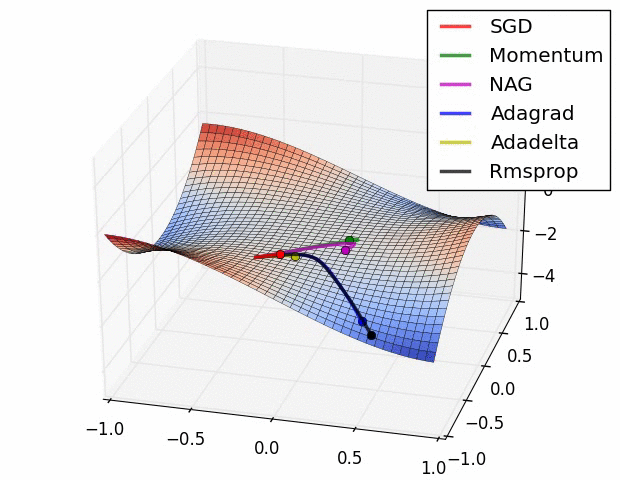
\includegraphics[width = .49\textwidth]{figure/sattle_point2-50.png}}
      \href{https://giphy.com/embed/SJVFO3IcVC0M0}{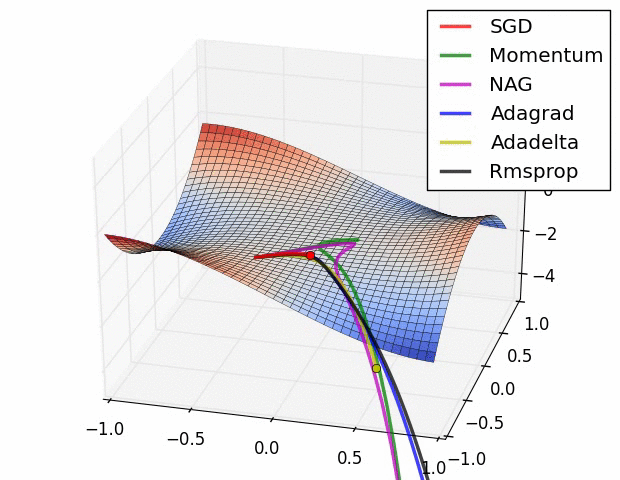
\includegraphics[width = .49\textwidth]{figure/sattle_point2-150.png}}
      \tiny{\\Credits: Dettmers (2015) and Radford}
      \end{center}
      \caption{Excerpts from an animation to compare the behavior of momentum and
      other methods compared to SGD for a saddle point. Left: After a few seconds; Right: A bit later. The animation shows that all showed methods accelerate optimization compared to the standard SGD. The highest acceleration is obtained using Rmsprop followed by Adagrad as learning rate strategies. You can find the animation \href{https://giphy.com/embed/SJVFO3IcVC0M0}{\textcolor{blue}{here}} or click on the images above.}
    \end{figure}
}
 
%%%%%%%%%%%%%%%%%%%%%%%%%%%%%%%%%%%%%%%%%%%%%%%%%%%%%%%%%%%%%%%%

% \begin{vbframe}{Batch normalization}
% \textbf{Motivation:}
% 
% As shown earlier, neural networks learn a nonlinear transformation of the input space such that in the last layer(s), a simple classification is sufficient to seperate our data well.
% To do so, especially in deep networks, we need to coordinate updates between the layers.
% Batch normalization forces the model to learn a nonlinear transformation in a layer by removing changes in mean and standard deviation from the layers output.
% 
% \framebreak
%   \begin{itemize}
%     \item Batch Normalization is no algorithm, but rather a technique to improve optimization in certain situations.
%     \item It is an extra component that can be placed between each layer of the neural network.
%     \item That component takes the activation of the antecedent layer and normalizes it before sending it to the next \enquote{actual layer}.
%     $$ H' = \frac{H-\mu}{\sigma}$$
%     with $H$ being the activated minibatch of the previous layer, $\mu$ the mean and $\sigma$ the standard deviation of each unit.
%   \end{itemize}
% \framebreak
%   \begin{itemize}
%     \item For our final benchmark in this chapter we compute two models to predict the mnist data.
%     \item One will extend our basic architecture such that we add batch normalization to all hidden layers.
%     \item We use SGD as optimizer with $momentum = 0.9$, $learning.rate = 0.03$ and $wd = 0.001$.
%     \item []
% <<mxnet3, size = "scriptsize", cache = TRUE, eval = FALSE, echo = TRUE>>=
% fc1 = mx.symbol.FullyConnected(data, num_hidden = 512)
% act1 = mx.symbol.Activation(fc1, act_type = "relu")
% bn1 = mx.symbol.BatchNorm(act1)
% fc2 = mx.symbol.FullyConnected(bn1, num_hidden = 512)
% act2 = mx.symbol.Activation(fc2, act_type = "relu")
% bn2 = mx.symbol.BatchNorm(act2)
% fc3 = mx.symbol.FullyConnected(bn2, num_hidden = 512)
% act3 = mx.symbol.Activation(fc3, act_type = "relu")
% bn3 = mx.symbol.BatchNorm(act3)
% fc4 = mx.symbol.FullyConnected(bn3, num_hidden = 10)
% softmax = mx.symbol.SoftmaxOutput(fc4, name = "sm")
% @
%   \end{itemize}
% \framebreak
%   \begin{figure}
%   \centering
%     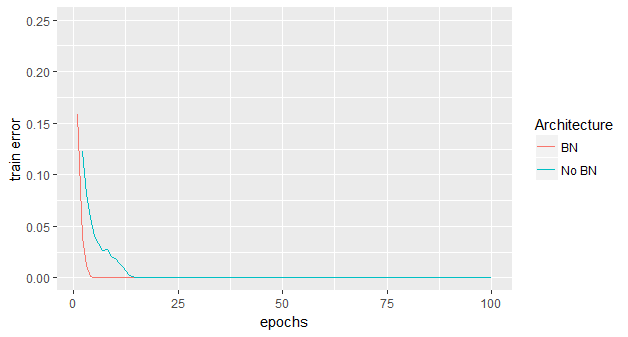
\includegraphics[width=12cm]{figure/bnTrain.png}
%   \end{figure}
% \framebreak
%   \begin{figure}
%   \centering
%     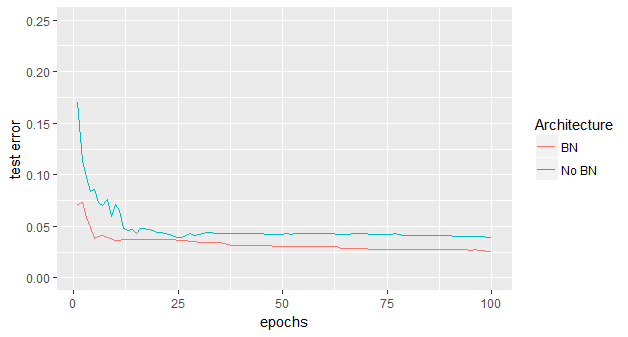
\includegraphics[width=12cm]{figure/bnTest.png}
%   \end{figure}
% \end{vbframe}
%%%%%%%%%%%%%%%%%%%%%%%%%%%%%%%%%%%%%%%%%%%%%%%%%%%%%%%%%%%%%%%%%%
\section{Batch Normalization}

\begin{frame} {Batch Normalization}
  \begin{itemize}
    \item Batch Normalization (BatchNorm) is an extremely popular technique that improves the training speed and stability of deep neural nets.
    \item It is an extra component that can be placed between each layer of the neural network.
    \item It works by changing the "distribution" of activations at each hidden layer of the network.
    \item We know that it is sometimes beneficial to normalize the inputs to a learning algorithm by shifting and scaling all the features so that they have 0 mean and unit variance.
    \item% Analogously,
     BatchNorm applies a similar transformation to the activations of the hidden layers (with a couple of additional tricks).
  \end{itemize}
\end{frame}

\begin{frame} {Batch Normalization}
  \begin{itemize}
    \item For a hidden layer with neurons $z_j$, $j=1, \dots, J$, BatchNorm is applied to each $z_j$ by considering the activations of $z_j$ \textbf{over a given minibatch} of inputs.
    \item Let $z_j^{(i)}$ denote the activation of $z_j$ for input $x^{(i)}$ in the minibatch (of size $m$).
    \item The mean and variance of the activations are
      \begin{equation*}
          \begin{array}{l}
            \mu_j = \frac{1}{m} \sum \limits_i \limits^m z_j^{(i)} \\
            \sigma^2_j = \frac{1}{m} \sum \limits_i \limits^m (z_j^{(i)} - \mu_j)^2
          \end{array}
      \end{equation*}
    \item Each $z_j^{(i)}$ is then normalized 
        \begin{equation*}
          \tilde z_j^{(i)} = \frac {z_j^{(i)} - \mu_j}{\sqrt{\sigma^2_j + \epsilon}}
        \end{equation*}
        where a small constant, $\epsilon$, is added for numerical stability.
  \end{itemize}
\end{frame}


\begin{frame} {Batch Normalization}
  \begin{itemize}
    \item It may not be desirable to normalize the activations in such a rigid way because potentially useful information can be lost in the process.
    \item Therefore, we commonly let the training algorithm decide the "right amount" of normalization by allowing it to re-shift and re-scale $\tilde z_j^{(i)}$ to arrive at the batch normalized activation $\hat z_j^{(i)}$:
        \begin{equation*}
          \hat z_j^{(i)} = \gamma_j \tilde z_j^{(i)} + \beta_j
        \end{equation*}
    \item $\gamma_j$ and $\beta_j$ are learnable parameters that are also tweaked by backpropogation.
    \item $\hat z_j^{(i)}$ then becomes the input to the next layer.
    \item Note: The algorithm is free to scale and shift each $\tilde z_j^{(i)}$ back to its original (unnormalized) value.
  \end{itemize}
\end{frame}

\begin{frame} {Batch Normalization: Illustration}
  \begin{itemize}
    \item Recall: $z_j = \sigma(W_j^T x + b_j)$
    \item So far, we have applied batch-norm to the activation $z_j$. It is possible (and more common) to apply batch norm to $W_j^Tx + b_j$ \textit{before} passing it to the nonlinear activation $\sigma$.
  \end{itemize}
    \begin{figure}
    \centering
      \scalebox{0.32}{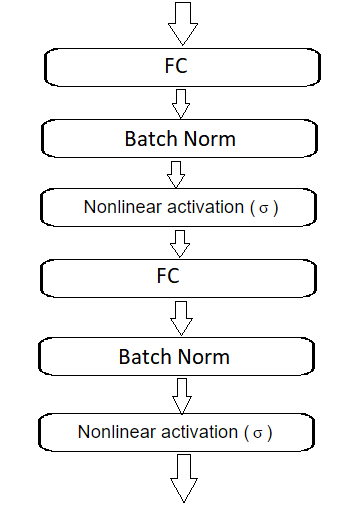
\includegraphics{figure/batchy.png}}
      \caption{\footnotesize FC = Fully Connected layer. BatchNorm is applied \textit{before} the nonlinear activation function.}
  \end{figure}
\end {frame}

%%%%%%%%%%%%%%%%%%%%%%%%%%%%%%%%%%%%%%%%%%%%%%%%%%


\begin{frame} {Batch Normalization}
  \begin{itemize}
    \item The key impact of BatchNorm on the training process is this: It reparametrizes the underlying optimization problem to \textbf{make its landscape significantly more smooth}.
    \item One aspect of this is that the loss changes at a smaller rate and the magnitudes of the gradients are also smaller (see Santurkar et al. 2018).
  \end{itemize}
  \begin{figure}
    \centering
      \scalebox{0.6}{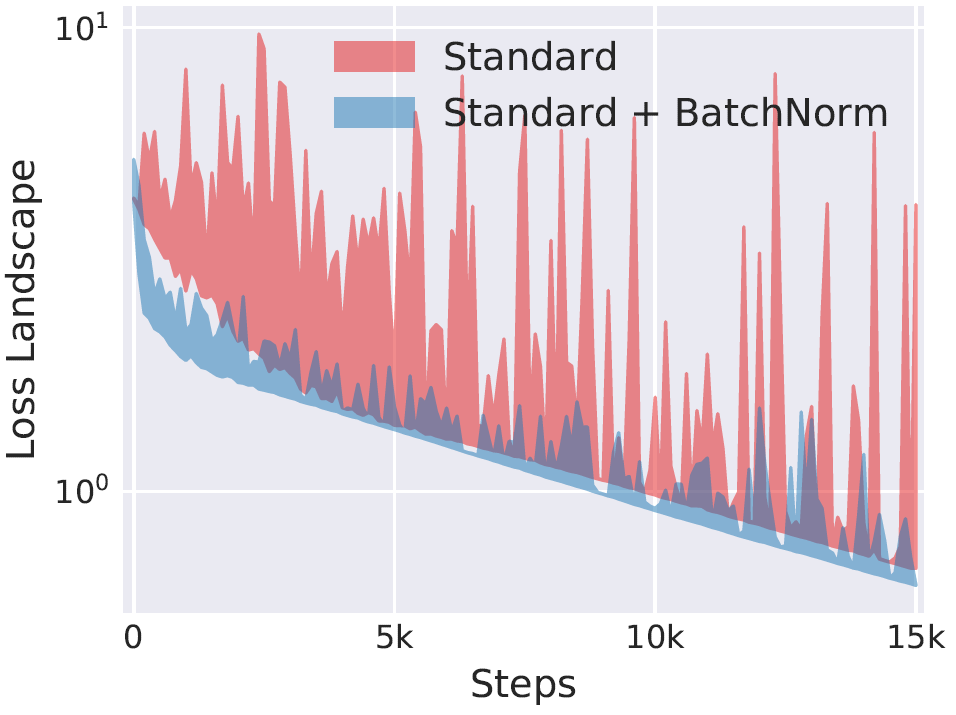
\includegraphics{figure/bn_effect.png}}
  \end{figure}
\end{frame}

\begin{frame} {Batch Normalization: Prediction}
  \begin{itemize}
    \item Once the network has been trained, how can we generate a prediction for a single input (either at test time or in production)?
    \item One option is to feed the entire training set to the (trained) network and compute the means and standard deviations.
    \item More commonly, during training, an exponentially weighted running average of each of these statistics over the minibatches is maintained.
    \item The learned $\gamma$ and $\beta$ parameters are then used (in conjunction with the running averages) to generate the output.
  \end{itemize}
\end{frame}

\begin{vbframe}{Batch Normalization}
\begin{itemize}
    \item For our final benchmark in this chapter we compute two models to predict the mnist data.
    \item One will extend our basic architecture such that we add batch normalization to all hidden layers.
    \item We use SGD as optimizer with  a momentum of 0.9, a learning rate of 0.03 and weight decay of 0.001.
  \end{itemize}

\framebreak


  \begin{figure}
  \centering
    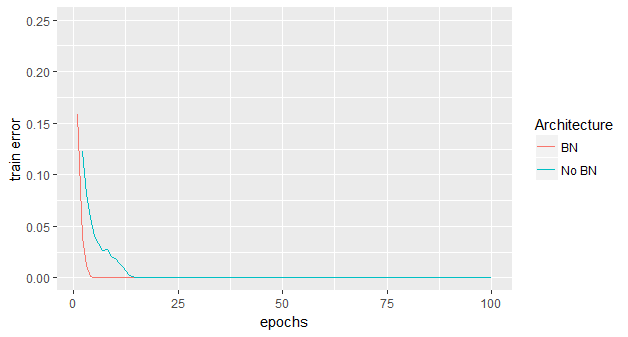
\includegraphics[width=12cm]{figure/bnTrain.png}
  \end{figure}
  Batch Normalization accelerated learning. 
  
  
\framebreak
  
  \begin{figure}
  \centering
    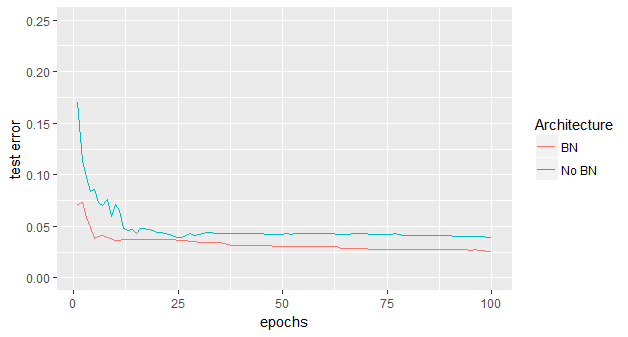
\includegraphics[width=12cm]{figure/bnTest.png}
  \end{figure}
  Batch Normalization resulted in a lower test error. 
\end{vbframe}

%%%%%%%%%%%%%%%%%%%%%%%%%%%%%%%%%%%%%%%%%%%%%%%%%%%%%%%%%%%%%%%%%%
% \begin{vbframe}{Second order optimization}
%   \begin{itemize}
%     \item Second order optimization methods include information about the curvature but require computing the Hessian matrix.
%       \begin{itemize}
%         \item Very expensive for large networks!
%         \item Think of the network we applied in the regularization chapter:
%       \end{itemize}
%     \begin{figure}
%       \centering
%         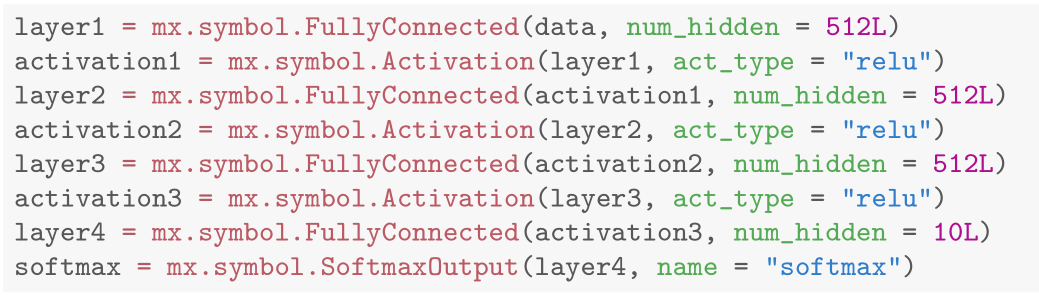
\includegraphics[width=8cm]{figure/mxnet_regulariation_1.png}
%     \end{figure}
%     \item This model has a huge amount of parameters:
%     \begin{eqnarray*}
%       &=& \underbrace{784 \cdot 512}_{\text{input to 1st layer}} + \underbrace{512^2}_{\text{1st to 2nd layer}} + \underbrace{512^2}_{\text{2nd to 3rd layer}} + \underbrace{512 \cdot 10}_{\text{3rd to output}} \\
%       &=& 3.285.504
%     \end{eqnarray*}
%   \end{itemize}
% \framebreak
%   \begin{itemize}
%     \item A first order method would need $3.285.504$ partial derivatives to compute the gradients.
%     \item Second order methods on the other hand require $$3.285.504^2 = 10.794.536.534.016$$ partial derivatives!
%     \item For small problems/networks one might consider the BFGS (Broyden-Fletcher-Goldfarb-Shanno) algorithm, which computes an approximation of the Hessian (still expensive!).
%       \begin{itemize}
%         \item Very difficult to implement, alot of programming know-how necessary to create an efficient implementation.
%       \end{itemize}
%     \item For huge networks even gradient descent becomes too expensive.
%       \begin{itemize}
%         \item Solution: parameters are instead grouped into mini-batches (stochastic gradient descent)
%       \end{itemize}
%   \end{itemize}
% \end{vbframe}


%%%%%%%%%%%%%%%%%%%%%%%%%%%%%%%%%%%%%%%%%%%%%%%%%%%%%%%%%%%%%%%%%%
%%%%%%%%%%%%%%%%%%          REFERENCES          %%%%%%%%%%%%%%%%%%
%%%%%%%%%%%%%%%%%%%%%%%%%%%%%%%%%%%%%%%%%%%%%%%%%%%%%%%%%%%%%%%%%%
\begin{vbframe}
\frametitle{References}
\footnotesize{
\begin{thebibliography}{99}
%%%%%%%%%%%%%%%%%%%%%%%%%%%%%%%%%%
\bibitem[Ian Goodfellow et al., 2016]{1} Ian Goodfellow, Yoshua Bengio and Aaron Courville (2016)
\newblock Deep Learning
\newblock \emph{\url{http://www.deeplearningbook.org/}}
%%%%%%%%%%%%%%%%%%%%%%%%%%%%%%%%%%
\bibitem[Yann Dauphin et al., 2014]{2} Yann Dauphin, Razvan Pascanu, {\c{C}}aglar G{\"{u}}l{\c{c}}ehre, Kyunghyun Cho, Surya Ganguli, Yoshua Bengio (2014)
\newblock Identifying and attacking the saddle point problem in high-dimensional non-convex optimization
\newblock \emph{\url{https://arxiv.org/abs/1406.2572}}
%%%%%%%%%%%%%%%%%%%%%%%%%%%%%%%%%%
\bibitem[Hao Li et al., 2017]{3} Hao Li, Zheng Xu, Gavin Taylor, Christoph Studer, Tom Goldstein (2017)
\newblock Visualizing the Loss Landscape of Neural Nets
\newblock \emph{\url{https://arxiv.org/abs/1712.09913}}
%%%%%%%%%%%%%%%%%%%%%%%%%%%%%%%%%
\bibitem[Tim Dettmers, 2015]{4} Tim Dettmers (2015)
\newblock Deep Learning in a Nutshell: History and Training
\newblock \emph{\url{https://devblogs.nvidia.com/deep-learning-nutshell-history-training/}}
%%%%%%%%%%%%%%%%%%%%%%%%%%%%%%%%%
\bibitem[Hafidz Zulkifli, 2018]{5} Hafidz Zulkifli (2018)
\newblock Understanding Learning Rates and How It Improves Performance in Deep Learning
\newblock \emph{\url{https://towardsdatascience.com}}
%%%%%%%%%%%%%%%%%%%%%%%%%%%%%%%%%
\bibitem[Loshchilov, Hutterer, 2016]{6} Ilya Loshchilov, Frank Hutter (2016)
\newblock SGDR: Stochastic Gradient Descent with Warm Restarts
\newblock \emph{\url{https://arxiv.org/abs/1608.03983}}
%%%%%%%%%%%%%%%%%%%%%%%%%%%%%%%%%
\bibitem[Jeremy Jordan, 2018]{7} Jeremy Jordan (2018)
\newblock Setting the learning rate of your neural network
\newblock \emph{\url{https://www.jeremyjordan.me/nn-learning-rate/}}
%%%%%%%%%%%%%%%%%%%%%%%%%%%%%%%%%
\bibitem[Santurkar et al. 2018]{8} Shibani Santurkar, Dimitris Tsipras, Andrew Ilyas, Aleksander Madry (2018)
\newblock How Does Batch Normalization Help Optimization?
\newblock \emph{\url{https://arxiv.org/abs/1805.11604}}
%%%%%%%%%%%%%%%%%%%%%%%%%%%%%%%%%
\bibitem[Akshay Chandra 2015]{9} Akshay Chandra (2015) 
\newblock Learning Parameters, Part 2: Momentum-Based \& Nesterov Accelerated Gradient Descent
\newblock \emph{\url{https://towardsdatascience.com/learning-parameters-part-2-a190bef2d12}}
\end{thebibliography}
}
\end{vbframe}

\endlecture
\end{document}










